\chapter{Numerical Experiments II: The Bottom Rung}
\label{ch:experiments2}

Chapter~\ref{ch:experiments} ended by describing the experiment it had not done: the mixing time\index{mixing time} of the bottom rung chain as a function of $N$. This chapter does it for the swap chain on unconditioned boards up to $N = 32$. The result is that the autocorrelation time grows like $N^{1.8}$ over this range, which is polynomial, and the ratio $Z_0 / Z_1$ estimated from the chain decreases roughly like $0.5/N$ over this range, so that the data do not show a positive limit. On unconditioned boards, at these sizes, the bottom rung is not stuck.

\section{Design}

For each $N$ in $\{ 8, 10, 12, 14, 16, 18, 20, 24, 28, 32 \}$ a solution was found by a min conflicts heuristic, and the swap chain on $\{ S \le 1 \}$ was run from it for $4000 N$ proposed swaps, recording at each step the column $x_1$ of the queen in the first row. The integrated autocorrelation time of this sequence,
\[
\tau_{\rm int} = 1 + 2 \sum_{k \ge 1} \mathrm{corr}(x_1(t), x_1(t + k)) ,
\]
was estimated with the sum truncated where the correlation first falls below $0.02$. The statistic $x_1$ was chosen because it is a coordinate of the configuration that must be decorrelated for the chain to have mixed, and because it is cheap; the column of any row would do. Six independent runs from six independent starting solutions were made at each $N$ and the mean and standard deviation of $\tau_{\rm int}$ recorded. A separate run of $2000 N$ steps recorded the fraction of time the chain spent at energy zero, which estimates $Z_0 / Z_1 = N(0) / (N(0) + N(1))$.

\section{Results}

\begin{table}[t]
\centering
\small
\caption{Integrated autocorrelation time of the first row column under the swap chain on $\{ S \le 1 \}$, in proposed swaps, mean and standard deviation over six runs; and the fraction of time at energy zero.}
\label{tab:mixing}
\begin{tabular}{rrrr}
\toprule
$N$ & $\tau_{\rm int}$ mean & $\tau_{\rm int}$ sd & fraction at $S = 0$ \\
\midrule
8 & 59 & 10 & 0.094 \\
10 & 168 & 31 & 0.061 \\
12 & 297 & 82 & 0.034 \\
14 & 423 & 128 & 0.044 \\
16 & 430 & 166 & 0.032 \\
18 & 398 & 29 & 0.023 \\
20 & 528 & 62 & 0.022 \\
24 & 994 & 544 & 0.019 \\
28 & 723 & 169 & 0.014 \\
32 & 928 & 101 & 0.018 \\
\bottomrule
\end{tabular}
\end{table}

\begin{figure}[t]
\centering
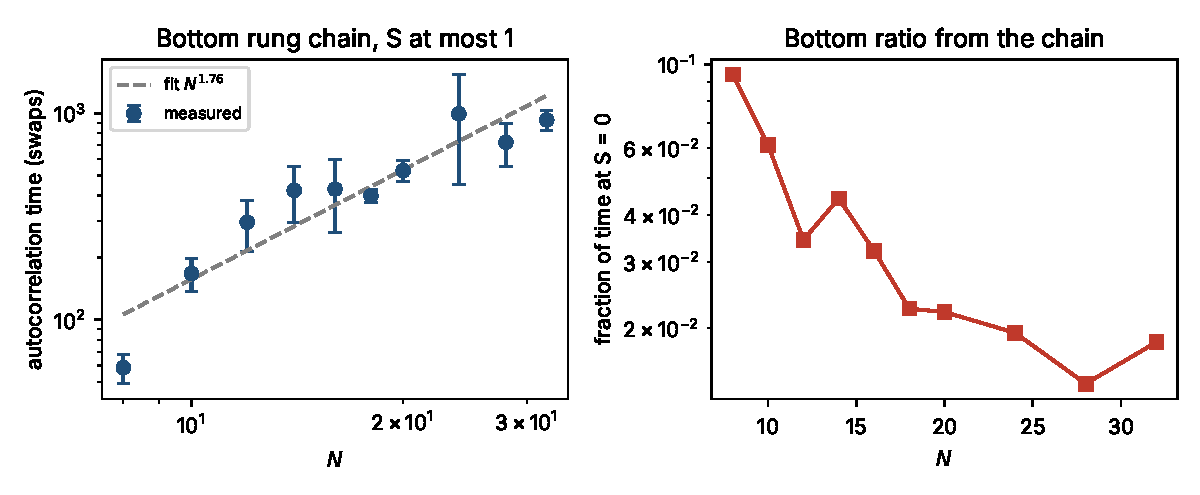
\includegraphics[width=\textwidth]{fig_mixing.pdf}
\caption{Left: autocorrelation time of the bottom rung chain against $N$ on logarithmic axes, with a power law fit of exponent $1.76$. Right: the fraction of time at energy zero, which estimates $Z_0 / Z_1$.}
\label{fig:mixing}
\end{figure}

Table~\ref{tab:mixing} and Figure~\ref{fig:mixing} give the results. The autocorrelation time grows from $59$ swaps at $N = 8$ to about $900$ at $N = 32$, and a power law fit on logarithmic axes gives an exponent of $1.76$ with no clear curvature given the scatter. The fraction of time at energy zero, which is the bottom ratio of the ladder, falls from $0.094$ at $N = 8$, where the exact value is $92 / (92 + 888) = 0.094$, to about $0.015$ at $N = 28$ to $32$, and its product with $N$ stays between $0.4$ and $0.75$, so the decrease is consistent with decay like $1/N$ and the data do not show a positive limit.

\section{Interpretation}

Three readings.

First, the swap chain on $\{ S \le 1 \}$ for unconditioned boards does mix, in the sense that the first row column decorrelates in a number of steps polynomial in $N$ over the range tested. Since each proposed swap costs $O(N)$ to evaluate incrementally, the cost of an effectively independent sample is $O(N^{2.8})$, and the cost of the bottom rung of the ladder with $M$ samples is $O(M N^{2.8})$. With $M = O(N / \epsilon^2)$, which assumes the bottom ratio is bounded below and which the data above do not show, from the product estimator\index{product estimator} bound this is $O(N^{3.8} / \epsilon^2)$ for the bottom rung, and the whole ladder is $O(N)$ rungs each cheaper than the bottom, so the walk on unconditioned boards costs $O(N^{4.8} / \epsilon^2)$ if the exponent holds. This is an extrapolated cost estimate, not a demonstrated polynomial algorithm: the counts were checked against exact values only to $N = 16$, the exponent is measured on a finite range, and the estimate assumes that the upper rungs are cheaper than the bottom one. The relaxation times of Chapter~\ref{ch:open} grow faster, like $N^3$, which would raise the exponent.

Second, this says nothing about the completion problem on hard instances, which is where the $\NP$ hardness is. The unconditioned level set $\{ S \le 1 \}$ contains all $Q(N)$ solutions together with the $N(1)$ placements with one attacking pair, and since $Q(N)$ grows like $N!$ times $e^{-0.942 N}$ up to subexponential factors there are a great many solutions, spread through the permutation group, and the one attack placements serve as bridges between them. On a conditioned board with few free rows, or on a reduction board where the free squares are a sparse pattern designed to encode a formula, the level set is small and its connectivity under swaps is a different question entirely. The experiment is consistent with the first half of the conjecture of Chapter~\ref{ch:swendsen}, though it concerns the swap chain and not the block chain. The exact connectivity computations of Chapter~\ref{ch:open} extend the support to boards conditioned on queens of a random solution, up to $N = 17$, where the giant component\index{giant component} of completions survives; they are silent on adversarially conditioned boards.

Third, the ratio $Z_0 / Z_1$ decreases slowly with $N$, and the data do not settle whether the number of placements with exactly one attacking pair is a bounded multiple of the number of solutions: the implied ratio $N(1)/N(0)$ rises from about $10$ at $N = 8$ to roughly $50$ to $70$ at the largest $N$, with no sign of saturating. This is a statement about the solution landscape: on average a solution is surrounded by a polynomial number of near solutions, which is why the swap chain can move, and it suggests that the bottom rung could be replaced by a direct count of near solutions per solution if that multiple could be computed. We leave this as an open problem.

\section{What would change the picture}

A further experiment would sharpen the picture considerably, and it is within reach of a laptop.

Run the same chain on reduction boards. Take a small hard satisfiability instance, apply the Gent Jefferson Nightingale~\cite{GJN} construction to obtain a board and a partial placement, and run the swap chain on the level set $\{ S \le 1 \}$ of the free rows. If the autocorrelation time explodes, or the chain fails to leave the component it starts in, the second half of the conjecture is supported. The construction is intricate and we have not implemented it; doing so is the most valuable next step in the program.

\section{Summary}

On unconditioned boards the bottom rung autocorrelation time grows like $N^{1.8}$ up to $N = 32$, which under the assumptions above extrapolates to a cost near $N^5$ for the vertical walk; the counts themselves were checked against exact values only to $N = 16$. This is the first measurement of the mixing of the queens level set chain that we know of, and it suggests that for the unconditioned problem the Monte Carlo program works at these sizes. For the completion problem on hard boards, which is the problem whose solution in randomized polynomial time would give $\NP = \RP$, we have no measurement. What we have, from the exact computations of Chapter~\ref{ch:open}, is the measurement on boards conditioned on randomly placed queens at $N = 12$, a pointer rather than a result: the bottom level set appears to shatter there, so that the chain of this chapter would be trapped, but the level set three or four attacks up is connected, so that the walk with the bottom rungs skipped would not be. On random boards the typical depth has since been measured to move by about one, from 3 at $N = 12$ to 4 at $N = 16$, which the data do not yet show to be growth (Section~\ref{sec:round4} of Chapter~\ref{ch:open}). The question for hard boards is whether the depth stays bounded or grows with $N$, and we expect, when that measurement is made, that it grows.
